% appendix_figures.tex
% Core v2.5 — Appendix G: Figures, Diagrams, and Structural Maps

\section{Appendix G: Figures and Structural Maps}
\label{sec:appendix-figures}

This appendix collects all high-level structural diagrams used
throughout the Continuum Framework.  
All figures are provided in TikZ form to ensure full reproducibility,
portability, and consistency with scientific publishing standards.

The diagrams included here correspond to the core transitions,
universal architecture, and level hierarchy.

% -------------------------------------------------
% Figure 1 — Universal Architecture of a Continuum
% -------------------------------------------------

\begin{figure}[h!]
\centering
\begin{tikzpicture}[node distance=1.4cm, >=stealth]

% Nodes
\node[draw, rounded corners, thick, fill=gray!5, inner sep=8pt]
  (omega) {$\Omega(K)$};
\node[draw, rounded corners, thick, right=3.1cm of omega,
  fill=gray!5, inner sep=8pt]
  (boundary) {$\partial \Omega(K)$};

\node[draw, rounded corners, thick, above left=1.4cm and -0.3cm of omega,
  fill=gray!5] (A) {$A$};
\node[draw, rounded corners, thick, above=1.4cm of omega,
  fill=gray!5] (P) {$P$};
\node[draw, rounded corners, thick, above right=1.4cm and -0.3cm of omega,
  fill=gray!5] (Theta) {$\Theta$};

\node[draw, rounded corners, thick, below left=1.4cm and -0.3cm of omega,
  fill=gray!5] (J) {$J$};
\node[draw, rounded corners, thick, below=1.4cm of omega,
  fill=gray!5] (C) {$C$};
\node[draw, rounded corners, thick, below right=1.4cm and -0.3cm of omega,
  fill=gray!5] (k) {$k$};

% Arrows
\draw[->, thick] (A) -- (omega);
\draw[->, thick] (P) -- (omega);
\draw[->, thick] (Theta) -- (omega);
\draw[->, thick] (J) -- (omega);
\draw[->, thick] (C) -- (omega);
\draw[->, thick] (k) -- (omega);

% Boundary arrow
\draw[->, thick, red] (omega) -- node[above]{critical} (boundary);

\end{tikzpicture}
\caption{Universal architecture of a continuum \(K\).}
\label{fig:architecture}
\end{figure}

% -------------------------------------------------
% Figure 2 — Transition Operator Ψₓ→ₓ₊₁
% -------------------------------------------------

\begin{figure}[h!]
\centering
\begin{tikzpicture}[>=stealth, node distance=2.2cm, thick]

\node[draw, rounded corners, fill=gray!7, minimum width=2.9cm,
  minimum height=1.3cm] (Kx) {$K_x$};
\node[draw, rounded corners, fill=gray!7, right=4cm of Kx,
  minimum width=2.9cm, minimum height=1.3cm] (Kx1) {$K_{x+1}$};

\draw[->, blue, thick] (Kx) -- node[above, black]
  {$\Psi_{x\rightarrow x+1}$} (Kx1);

\end{tikzpicture}
\caption{Transition operator \(\Psi_{x\rightarrow x+1}\).}
\label{fig:psi}
\end{figure}

% -------------------------------------------------
% Figure 3 — Hierarchical Levels K₀–K₁₂
% -------------------------------------------------

\begin{figure}[h!]
\centering
\begin{tikzpicture}[node distance=1.1cm, thick]

\node[draw, rounded corners, fill=gray!10] (K0) {$K_0$};
\node[draw, rounded corners, fill=gray!10, below=of K0] (K1) {$K_1$};
\node[draw, rounded corners, fill=gray!10, below=of K1] (K2) {$K_2$};
\node[draw, rounded corners, fill=gray!10, below=of K2] (K3) {$K_3$};
\node[draw, rounded corners, fill=gray!10, below=of K3] (K4) {$K_4$};
\node[draw, rounded corners, fill=gray!10, below=of K4] (K5) {$K_5$};
\node[draw, rounded corners, fill=gray!10, below=of K5] (K6) {$K_6$};
\node[draw, rounded corners, fill=gray!10, below=of K6] (K7) {$K_7$};
\node[draw, rounded corners, fill=gray!10, below=of K7] (K8) {$K_8$};
\node[draw, rounded corners, fill=gray!10, below=of K8] (K9) {$K_9$};
\node[draw, rounded corners, fill=gray!10, below=of K9] (K10) {$K_{10}$};
\node[draw, rounded corners, fill=gray!10, below=of K10] (K11) {$K_{11}$};
\node[draw, rounded corners, fill=gray!10, below=of K11] (K12) {$K_{12}$};

\foreach \a/\b in {K0/K1, K1/K2, K2/K3, K3/K4, K4/K5, K5/K6,
                   K6/K7, K7/K8, K8/K9, K9/K10, K10/K11, K11/K12}
{
  \draw[->, blue] (\a) -- (\b);
}

\end{tikzpicture}
\caption{Hierarchy of continua \(K_0\) through \(K_{12}\).}
\label{fig:hierarchy}
\end{figure}

% -------------------------------------------------
% Figure 4 — Boundary ∂Ω as Threshold Surface
% -------------------------------------------------

\begin{figure}[h!]
\centering
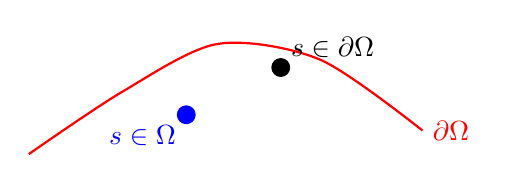
\begin{tikzpicture}[>=stealth, thick]

% Boundary curve
\draw[red, thick, smooth] plot coordinates {
  (0,0.3) (1.2,1.1) (2.4,1.7) (3.7,1.5) (5,0.6)
} node[right] {$\partial\Omega$};

% Points inside
\filldraw[blue] (2,0.8) circle (3pt) node[below left] {$s\in\Omega$};
\filldraw[black] (3.2,1.4) circle (3pt) node[above right] {$s\in\partial\Omega$};

\end{tikzpicture}
\caption{The admissibility boundary \(\partial\Omega\).}
\label{fig:boundary}
\end{figure}

% -------------------------------------------------
% Figure 5 — Cycle Structure Cₙ
% -------------------------------------------------

\begin{figure}[h!]
\centering
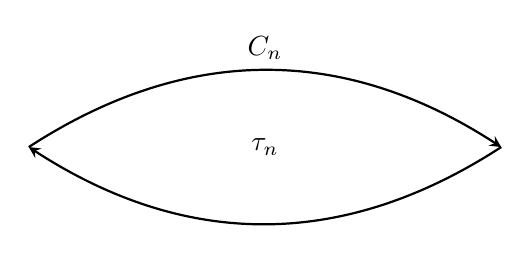
\begin{tikzpicture}[>=stealth, thick]

\draw[->] (0,0) .. controls (2,1.3) and (4,1.3) .. (6,0)
           node[midway, above] {$C_n$};
\draw[->] (6,0) .. controls (4,-1.3) and (2,-1.3) .. (0,0);

\node at (3,0) {$\tau_n$};

\end{tikzpicture}
\caption{A generic cycle \(C_n\) with period \(\tau_n\).}
\label{fig:cycle}
\end{figure}

% -------------------------------------------------
% Summary
% -------------------------------------------------

\section*{Summary}

This appendix provides TikZ-based diagrams for:

\begin{itemize}
  \item universal continuum architecture,
  \item transition operator \(\Psi_{x\to x+1}\),
  \item hierarchical structure \(K_0\)–\(K_{12}\),
  \item admissibility boundary \(\partial\Omega\),
  \item cycle structure \(C_n\).
\end{itemize}

They form the visual backbone of the Continuum Framework and are fully
synchronised with Core v2.5.

